\section{Aufbau}
		
	\begin{figure}
		\centering
		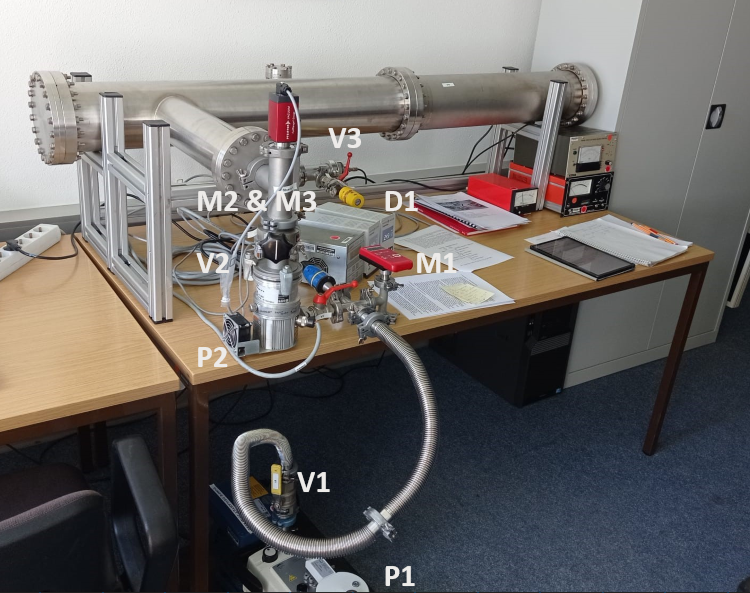
\includegraphics[width=0.8\textwidth]{"latex/images/Aufbau_beschriftet.png"}
		\caption{Ein Bild des verwendeten Versuchsaufbaus.}
		\label{fig:auf}
	\end{figure}		
	\noindent
	Beide in diesem Versuch verwendeten Vakuumpumpen sind in Abbildung \ref{fig:auf} zu sehen.\\
	Bei (P1) ist am unteren Ende des Bildes die Drehschiebervakuumpumpe zu sehen. 
	Die Turbomolekularpumpe ist direkt darüber auf dem Tisch bei (P2).\\
	Die Drehschieberpumpe kann mittels des Ventil (V1) und die Turbopumpe mittels des Ventil (V2) abgeschoben werden.
	Zwei weitere Ventile zum Einstellen des Gleichgewichtsdrucks sind das Ventil (V3) und das Dosierventil (D1) unter dem Vakuumkörper.\\
	Das erste relevante Messgerät ist bei (M1), welches ein kombiniertes Piezo und Pirani Vakuummeter ist.
	Bei (M2 \& M3) sind die Anzeigegeräte zu den Kaltkathoden-Vakuummetern, welche über der Turbopumpe (P2) und hinter dem Dosierventil (D1) angebracht sind.

\section{Durchführung}
	Zunächst wird die Funktionsfähigkeit der Anlage überprüft und vorbereitet. \\
	Dazu wird getestet, ob die Drehschieberpumpe (P1) innerhalb von maximal 10 Minuten in der Lage ist einen Enddruck $P_\text{E}$ von 0,03 mbar bis 0,05 mbar zu erzeugen. 
	Ist dem nicht so muss die Anlage auf undichte Stellen überprüft werden. \\
	Anschließend wird dann mit dem bereits vorhandenen Vorvakuum die Turbopumpe (P2) eingeschaltet.\\
	Um Wasseranlagerungen zu entfernen und Desorption vorzubeugen wird die Anlage auch einmal mit einem Heißluftföhn erhitzt.\\
	Die Turbopumpe sollte dann in der Lage sein, einen Druck von $\SI{8 e-5}{\milli\bar}$ bis $\SI{2 e-5}{\milli\bar}$ zu erzeugen.
	Weiterhin ist es sehr wichtig für die Auswertung einmal den Enddruck der Drehschieber- und Vakuumpumpe zu messen und zu dokumentieren.	


	\subsection{Messungen zur Drehschieberpumpe}

		Sobald bestätigt wurde, dass der Aufbau ausreichend dicht ist, können Evakuierungskurven aufgenommen und Leckratenmessungen durchgeführt werden.

		\subsubsection{Evakuierungskurve}

			Zunächst wird die Anlage wieder auf den Arbeitsbereich der Drehschieberpumpe belüftet. 
			Um Schäden an der Pumpe zu vermeiden, muss die Turbompumpe abgeschaltet werden. \\
			Dann wird die Drehschieberpumpe abgeschoben (V1) und der Rezipient belüftet, 
			indem für ca. 5 Sekunden das Dosierventil (D1) und Ventil (V3) geöffnet wird, 
			bis wieder Normaldruck in dem Rezipienten herrscht. \\
			Sobald der Rezipient wieder dicht ist, wird der Zugang zu der Drehschieberpumpe geöffnet (V1) und der Druckabfall als Funktion der Zeit vermessen. 
			Dazu werden für eine gesamte Messzeit von $\SI{600}{\second}$ alle $\SI{10}{\second}$ der Druck an dem digitalen Vakuummeter (M1) abgelesen.
			Bei dieser Messung sollte eine Enddruck von $P_\text{E}$ zwischen $\SI{0.1}{\milli\bar}$ und $\SI{0.08}{\milli\bar}$ erreicht werden.\\
			Diese Messung wird dann 3-mal wiederholt.

		\subsubsection{Leckratenmessung}

		 	Die Leckratenmessung wird durchgeführt, indem mittels des Nadelventils (D1) ein Gleichgewichtsdruck $p_\text{g}$ eingestellt und dann bei weiterhin offenem Dosierventil die Pumpe vom System abgeschoben wird (V1).\\
			Der darauf folgende Druckanstieg wird dann als Funktion der Zeit über $\SI{200}{\second}$ in $\SI{10}{\second}$ Abständen gemessen. \\
			Diese Messung wird mit 4 Gleichgewichtsdrücken $p_\text{g} = 0,4; 10; 40; \SI{80}{\milli\bar}$ und jeweils 3 Messreihen durchgeführt.

	\subsection{Messung zur Turbopumpe}

		Die Messungen zu der Turbopumpe (P2) laufen analog zu denen der Drehschieberpumpe ab. 
		Es ist hier wichtig darauf zu Achten, dass bevor die Turbopumpe eingeschaltet wird,
	    bereits eine Vorvakuum von mindestens $\SI{10e-1}{\milli\bar}$ mit der Drehschieberpumpe erzeugt wurde.
		
		\subsection{Evakuierungskurve}

			Dieses Mal wird der Rezipient nicht komplett belüftet, damit die Turbopumpe direkt starten kann. \\
			Als Startdruck  wird mit dem Dosierventil bei laufender Pumpe ein Druck von $\SI{1.6e-3}{\milli\bar}$ eingestellt.
			Dann wird das Ventil (V3) geschlossen und das zunehmende Vakuum in einer $p(t)$-Kurve über $\SI{200}{\second}$ alle $\SI{10}{\second}$ aufgenommen.\\
			Auch diese Messung wird 3-mal wiederholt.

		\subsection{Leckratenmessung}

			Die Leckratenmessungen der Turbopumpe läuft auch sehr analog zu denen der Drehschieberpumpe. \\
			Es werden lediglich nur über einen Zeitraum von $\SI{120}{\second}$ Werte aufgenommen.\\ 
			Die Gleichgewichtsdrücke hier, von denen die Leckratenmessung startet, sind: $(1\; \& \; 2)\cdot10^{-4} \; \si{\milli\bar}$ und $(5\; \& \; 7)\; \cdot10^{-5}\si{\milli\bar}$.\\
			Zum Abschiebern der Turbopumpe wird nun aber das Ventil (V2) verwendet.
